\documentclass[11pt,a4paper]{article}
\usepackage[utf8]{inputenc}
\usepackage[T1]{fontenc}
\usepackage[margin=1in]{geometry}
\usepackage{amsmath,amssymb,amsthm}
\usepackage{booktabs}
\usepackage{array}
\usepackage{enumitem}
\usepackage{fancyhdr}
\usepackage{hyperref}
\usepackage{listings}
\usepackage{xcolor}
\usepackage{tcolorbox}
\tcbuselibrary{breakable}
\usepackage{float}
\usepackage{tikz}
\usetikzlibrary{shapes.geometric, arrows.meta, positioning}

% Colors
\definecolor{codeblue}{rgb}{0.13,0.29,0.53}
\definecolor{backcolour}{rgb}{0.97,0.97,0.97}
\definecolor{asgbg}{rgb}{0.95,0.97,0.95}
\definecolor{asgborder}{rgb}{0.2,0.5,0.3}
\definecolor{warningbg}{rgb}{1.0,0.97,0.88}
\definecolor{warningborder}{rgb}{1.0,0.6,0.0}
\definecolor{lockdownbg}{rgb}{1.0,0.95,0.95}
\definecolor{lockdownborder}{rgb}{0.8,0.2,0.2}

% Theorem environments
\theoremstyle{definition}
\newtheorem{definition}{Definition}[section]
\newtheorem{invariant}{Invariant}[section]
\newtheorem{condition}{Condition}[section]
\theoremstyle{plain}
\newtheorem{theorem}{Theorem}[section]
\newtheorem{lemma}[theorem]{Lemma}

% Custom boxes
\newtcolorbox{asgbox}{colback=asgbg, colframe=asgborder, boxrule=1pt, title=Adaptive Spawn Governor}
\newtcolorbox{warningbox}{colback=warningbg, colframe=warningborder, boxrule=1pt, title=Caution}
\newtcolorbox{lockdownbox}{colback=lockdownbg, colframe=lockdownborder, boxrule=1pt, title=Emergency Lockdown}

% Code listings
\lstset{
    backgroundcolor=\color{backcolour},
    basicstyle=\ttfamily\footnotesize,
    keywordstyle=\color{codeblue}\bfseries,
    commentstyle=\color{gray},
    stringstyle=\color{purple},
    breaklines=true,
    frame=single,
    language=Python,
    showstringspaces=false
}

% Headers
\pagestyle{fancy}
\fancyhf{}
\fancyhead[L]{EFM Codex}
\fancyhead[R]{Appendix N v1.0}
\fancyfoot[C]{\thepage}
\setlength{\headheight}{14pt}

\title{
    {\Large\textsc{Entropica Forensic Model --- Appendix N}}\\[0.3cm]
    {\LARGE\bfseries Adaptive Spawn Governance}\\[0.2cm]
    {\Large Autonomous Parameter Calibration for Bounded Autonomy}\\[0.3cm]
    {\normalsize Version 1.2}
}
\author{Yology Research Division\\Entropica SPC}
\date{December 2025}

\begin{document}
\maketitle

\begin{abstract}
Appendix N specifies the \textbf{Adaptive Spawn Governor (ASG)}, an autonomous parameter calibration system that prevents spawn brittleness through continuous adaptation. Rather than hardcoding spawn parameters ($\tau_{spawn}$, $D_{max}$, $R_{max}$), the ASG observes swarm health metrics and adjusts parameters within profile-defined bounds. This enables self-healing behavior: a misconfigured or stressed swarm recovers within 50,000 ticks without human intervention, while preserving Gardener override authority (Commandment 4) through a rollback window. The ASG integrates with Appendix K (SHSL health metrics), Appendix I (deployment profiles), and Appendix M (Discovery Stack predictions).
\end{abstract}

\tableofcontents
\newpage

%==============================================================================
\section{Introduction}
%==============================================================================

\subsection{The Problem: Static Parameters}

Volume I v1.6 defines spawn conditions $S_1$--$S_6$ with hardcoded parameters:

\begin{table}[H]
\centering
\begin{tabular}{@{}lll@{}}
\toprule
\textbf{Parameter} & \textbf{Default} & \textbf{Function} \\
\midrule
$\tau_{spawn}$ & 0.7 & Minimum health to spawn \\
$D_{max}$ & 10 & Maximum lineage depth \\
$R_{max}$ & 100/tick & Global spawn rate limit \\
$R_{local,max}$ & 10/window & Per-parent spawn rate \\
\bottomrule
\end{tabular}
\caption{Static spawn parameters (Volume I §3.4).}
\end{table}

\textbf{Failure scenario:}
\begin{enumerate}[noitemsep]
    \item HFT swarm spawns at 85/tick (within $R_{max}$=100)
    \item Resource contention causes health drop: $0.75 \rightarrow 0.68 \rightarrow 0.62$
    \item Health falls below $\tau_{spawn}=0.7$
    \item \textbf{All spawning blocked}---system paralyzed
    \item Requires human intervention to adjust parameters
\end{enumerate}

\subsection{The Solution: Adaptive Calibration}

\begin{asgbox}
The Adaptive Spawn Governor (ASG) automatically calibrates parameters based on observed swarm behavior:
\begin{itemize}[noitemsep]
    \item Runs every $T_{calibration}=10,000$ ticks
    \item Reads metrics from Appendix K (SHSL)
    \item Adjusts parameters within profile bounds (Appendix I)
    \item Logs all adjustments to d-CTM (immutable audit)
    \item Gardener can rollback within $T_{review}=5,000$ ticks
\end{itemize}
\end{asgbox}

\subsection{Design Principles}

\begin{enumerate}
    \item \textbf{Bounded Adaptation:} Parameters never exceed profile bounds
    \item \textbf{Conservative Adjustment:} Faster to constrain, slower to loosen
    \item \textbf{Human Override:} Gardener rollback authority preserved
    \item \textbf{Full Accountability:} All adjustments logged to d-CTM
    \item \textbf{Hysteresis:} Cooldown prevents oscillation
\end{enumerate}

%==============================================================================
\section{Architecture}
%==============================================================================

\subsection{Component Overview}

\begin{center}
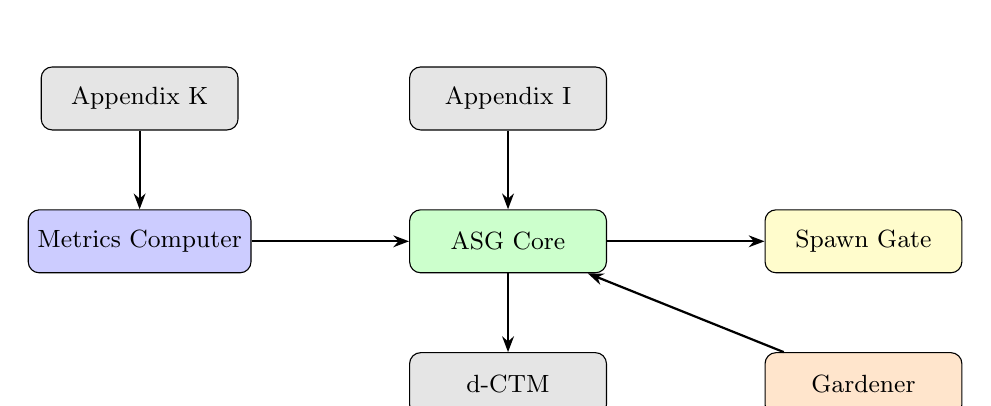
\begin{tikzpicture}[
    node distance=1cm,
    box/.style={rectangle, draw, rounded corners, minimum width=2.5cm, minimum height=0.8cm, font=\small},
    arrow/.style={-{Stealth[length=2mm]}, thick}
]

\node[box, fill=blue!20] (metrics) {Metrics Computer};
\node[box, fill=green!20, right=2cm of metrics] (asg) {ASG Core};
\node[box, fill=yellow!20, right=2cm of asg] (gate) {Spawn Gate};

\node[box, fill=gray!20, above=of metrics] (shsl) {Appendix K};
\node[box, fill=gray!20, above=of asg] (profiles) {Appendix I};
\node[box, fill=gray!20, below=of asg] (dctm) {d-CTM};
\node[box, fill=orange!20, below=of gate] (gardener) {Gardener};

\draw[arrow] (shsl) -- (metrics);
\draw[arrow] (metrics) -- (asg);
\draw[arrow] (profiles) -- (asg);
\draw[arrow] (asg) -- (gate);
\draw[arrow] (asg) -- (dctm);
\draw[arrow] (gardener) -- (asg);

\end{tikzpicture}
\end{center}

\subsection{Integration Points}

\begin{table}[H]
\centering
\begin{tabular}{@{}lll@{}}
\toprule
\textbf{Component} & \textbf{Interaction} & \textbf{Reference} \\
\midrule
Appendix K (SHSL) & ASG reads health metrics & §3.1 \\
Appendix I (Profiles) & ASG reads bounds & §4 \\
Appendix M (Discovery) & ASG receives predictions & §5.4 \\
Appendix L (Judicial) & Fork handling & §5.3 \\
d-CTM & Adjustment logging & §3.4 \\
Gardener & Rollback authority & §5.2 \\
\bottomrule
\end{tabular}
\end{table}

%==============================================================================
\section{Metrics Computation}
\label{sec:metrics}
%==============================================================================

\subsection{SwarmMetrics Data Structure}

\begin{definition}[SwarmMetrics]
The metrics computed every calibration cycle:
\begin{lstlisting}
@dataclass
class SwarmMetrics:
    avg_health: float          # Average health [0.0, 1.0]
    health_std_dev: float      # Health variance
    health_trend: float        # Change over last 10K ticks
    spawn_rate: float          # Capsules/tick (last 1000 ticks)
    vault_utilization: float   # Vault capacity used [0.0, 1.0]
    avg_depth: float           # Average lineage depth
    max_depth: int             # Maximum depth observed
    active_capsule_count: int  # Current active capsules
    anomaly_rate: float        # % with ANOMALY flags
\end{lstlisting}
\end{definition}

\subsection{Metrics Computation Algorithm}

\begin{lstlisting}[caption={MetricsComputer.compute\_metrics()}]
def compute_metrics(self, swarm_state) -> SwarmMetrics:
    """Extract metrics for calibration. O(n), <100ms for 10K capsules."""
    
    active_capsules = swarm_state.get_active_capsules()
    
    # Health metrics
    health_scores = [c.health for c in active_capsules]
    avg_health = statistics.mean(health_scores)
    health_std_dev = statistics.stdev(health_scores) if len(health_scores) > 1 else 0.0
    health_trend = avg_health - swarm_state.get_historical_health(ticks_ago=10000)
    
    # Spawn rate (last 1000 ticks)
    spawn_events = swarm_state.get_spawn_events(window=1000)
    spawn_rate = len(spawn_events) / 1000.0
    
    # Vault utilization
    total_capacity = swarm_state.vault.total_capacity
    allocated = sum(c.vault_allocation for c in active_capsules)
    vault_utilization = allocated / total_capacity
    
    # Depth metrics
    depths = [c.depth for c in active_capsules]
    avg_depth = statistics.mean(depths)
    max_depth = max(depths)
    
    # Anomaly rate
    anomalous = sum(1 for c in active_capsules if c.has_anomaly_flag())
    anomaly_rate = anomalous / len(active_capsules)
    
    return SwarmMetrics(...)
\end{lstlisting}

\subsection{Metrics Validation}

Before calibration proceeds, metrics are validated:

\begin{lstlisting}[caption={Metrics validation}]
def validate_metrics(self, metrics: SwarmMetrics) -> Tuple[bool, str]:
    checks = []
    if not (0.0 <= metrics.avg_health <= 1.0):
        checks.append(f"Invalid avg_health: {metrics.avg_health}")
    if metrics.spawn_rate < 0:
        checks.append(f"Invalid spawn_rate: {metrics.spawn_rate}")
    if not (0.0 <= metrics.vault_utilization <= 1.0):
        checks.append(f"Invalid vault_utilization: {metrics.vault_utilization}")
    if checks:
        return (False, "; ".join(checks))
    return (True, "All metrics valid")
\end{lstlisting}

\subsection{d-CTM Logging}

All metrics are logged to d-CTM for forensic reconstruction:

\begin{lstlisting}
log_to_dctm(
    event_type='ASG_METRICS',
    tick=current_tick,
    metrics=metrics,
    zk_sp_proof=generate_proof(metrics)
)
\end{lstlisting}

\subsubsection{Rich Observability (Gap 8)}

For operator debugging and trust, ASG logs comprehensive diagnostic context:

\begin{lstlisting}[caption={Rich diagnostic logging}]
def _log_calibration_with_diagnostics(self, adjustment, metrics, swarm_state):
    """Generate rich diagnostic context for operators."""
    
    diagnostics = {
        # Why did we adjust?
        'trigger': {
            'avg_health': metrics.avg_health,
            'health_threshold': 0.65,
            'spawn_rate': metrics.spawn_rate,
            'spawn_threshold': 0.8 * self.R_max,
            'vault_utilization': metrics.vault_utilization
        },
        
        # Which capsules are problematic?
        'top_spawners': swarm_state.get_top_spawners(n=10),
        'unhealthy_capsules': swarm_state.get_unhealthy(threshold=0.6, limit=20),
        
        # What do we expect to happen?
        'predicted_outcome': {
            'expected_health_in_10K': self._predict_health(metrics),
            'expected_recovery_ticks': self._estimate_recovery(metrics)
        },
        
        # Historical context
        'recent_adjustments': self.adjustment_history[-5:],
        'parameter_trajectory': self._get_param_trajectory(window=50000)
    }
    
    log_to_dctm(
        event_type='ASG_CALIBRATION',
        adjustment=adjustment,
        diagnostics=diagnostics,
        zk_sp_proof=generate_proof(adjustment, diagnostics)
    )
\end{lstlisting}

This enables operators to answer:
\begin{itemize}[noitemsep]
    \item \textbf{WHY} did ASG adjust? (trigger conditions)
    \item \textbf{WHICH} capsules are problematic? (top spawners, unhealthy list)
    \item \textbf{WHEN} will health improve? (predicted recovery time)
    \item \textbf{HOW} have parameters changed? (trajectory)
\end{itemize}

%==============================================================================
\section{Profile Bounds}
\label{sec:profiles}
%==============================================================================

\subsection{Bounded Adaptation}

ASG operates within \textbf{hard bounds} defined by deployment profile:

\begin{definition}[Adaptive Bounds]
\begin{equation}
\forall t: \begin{cases}
R_{min} \leq R_{max}(t) \leq R_{ceiling} \\
\tau_{min} \leq \tau_{spawn}(t) \leq \tau_{max} \\
D_{min} \leq D_{max}(t) \leq D_{ceiling}
\end{cases}
\end{equation}
\end{definition}

\subsection{Profile Definitions}

\begin{table}[H]
\centering
\small
\begin{tabular}{@{}lcccccc@{}}
\toprule
\textbf{Profile} & $R_{min}$ & $R_{ceiling}$ & $\tau_{min}$ & $\tau_{max}$ & $D_{min}$ & $D_{ceiling}$ \\
\midrule
SANDBOX & 10 & 1000 & 0.50 & 0.80 & 5 & 30 \\
PRODUCTION & 10 & 500 & 0.60 & 0.90 & 5 & 15 \\
CONTESTED & 5 & 100 & 0.70 & 0.95 & 3 & 8 \\
RESEARCH & 20 & 800 & 0.55 & 0.85 & 5 & 20 \\
\bottomrule
\end{tabular}
\caption{Adaptive bounds by deployment profile.}
\end{table}

\textbf{Profile rationale:}
\begin{itemize}[noitemsep]
    \item \textbf{SANDBOX:} Wide bounds for experimentation; failure acceptable
    \item \textbf{PRODUCTION:} Moderate bounds; stability critical
    \item \textbf{CONTESTED:} Tight bounds; under potential attack
    \item \textbf{RESEARCH:} Wide spawn capacity; probe deployment enabled
\end{itemize}

\subsection{Clamp Function}

\begin{lstlisting}[caption={Bound enforcement}]
def _clamp(self, value: float, min_val: float, max_val: float) -> float:
    """CRITICAL: Ensures value NEVER exceeds bounds."""
    return max(min_val, min(value, max_val))
\end{lstlisting}

%==============================================================================
\section{Calibration Algorithm}
\label{sec:calibration}
%==============================================================================

\subsection{Calibration Cycle}

\begin{lstlisting}[caption={Main calibration cycle}]
def calibrate_cycle(self, swarm_state, current_tick: int) -> List[Adjustment]:
    """Called every T_calibration=10,000 ticks."""
    
    # Step 0: Check cooldown (prevent oscillation)
    if current_tick - self.last_adjustment_tick < self.T_cooldown:
        return []  # Skip this cycle
    
    # Step 1: Compute metrics
    metrics = self.metrics_computer.compute_metrics(swarm_state)
    valid, reason = self.metrics_computer.validate_metrics(metrics)
    if not valid:
        log_warning(f"Invalid metrics: {reason}")
        return []
    
    # Step 2: Collect PROPOSED adjustments (don't apply yet)
    proposals = []
    proposals.extend(self._propose_health_adjustments(metrics, current_tick))
    proposals.extend(self._propose_resource_adjustments(metrics, current_tick))
    proposals.extend(self._propose_depth_adjustments(metrics, current_tick))
    
    # Step 3: Resolve conflicts (Gap 2)
    resolved = self._resolve_conflicts(proposals)
    
    # Step 4: Apply resolved adjustments
    for adj in resolved:
        self._apply_adjustment(adj)
        self._log_adjustment(adj)
    
    # Step 5: Update last adjustment tick
    if resolved:
        self.last_adjustment_tick = current_tick
    
    return resolved
\end{lstlisting}

\subsubsection{Multi-Parameter Conflict Resolution (Gap 2)}

When multiple adjustment sources propose changes to the same parameter, ASG resolves conflicts by priority:

\begin{lstlisting}[caption={Conflict resolution}]
def _resolve_conflicts(self, proposals: List[Adjustment]) -> List[Adjustment]:
    """
    If multiple proposals adjust same parameter, choose by priority.
    Safety-critical reasons take precedence over operational ones.
    """
    # Priority hierarchy (lower = higher priority)
    PRIORITY = {
        AdjustmentReason.RESOURCE_PRESSURE: 1,      # Safety-critical
        AdjustmentReason.APPROACHING_DEPTH_LIMIT: 2,
        AdjustmentReason.HIGH_SPAWN_LOW_HEALTH: 3,  # Operational
        AdjustmentReason.RAISE_HEALTH_BAR: 4,
        AdjustmentReason.HEALTHY_LOW_SPAWN: 5,      # Optimization
        AdjustmentReason.LOWER_HEALTH_BAR: 6,
        AdjustmentReason.SHALLOW_LINEAGES: 7,
        AdjustmentReason.UNDERUTILIZED: 8,
    }
    
    # Group proposals by parameter
    by_parameter = {}
    for proposal in proposals:
        param = proposal.parameter
        if param not in by_parameter:
            by_parameter[param] = []
        by_parameter[param].append(proposal)
    
    # Resolve each parameter
    resolved = []
    for param, competing in by_parameter.items():
        if len(competing) == 1:
            resolved.append(competing[0])
        else:
            # Multiple proposals: choose highest priority
            best = min(competing, key=lambda p: PRIORITY.get(p.reason, 99))
            resolved.append(best)
            
            # Log conflict resolution
            log_to_dctm(
                event_type='ASG_CONFLICT_RESOLVED',
                parameter=param,
                winner=best.reason,
                losers=[p.reason for p in competing if p != best]
            )
    
    return resolved
\end{lstlisting}

\textbf{Priority rationale:}
\begin{enumerate}[noitemsep]
    \item \textbf{RESOURCE\_PRESSURE} (highest): Vault exhaustion is safety-critical
    \item \textbf{APPROACHING\_DEPTH\_LIMIT}: Deep chains indicate potential attack
    \item \textbf{HIGH\_SPAWN\_LOW\_HEALTH}: System stability
    \item \textbf{Optimization reasons} (lowest): Can wait
\end{enumerate}

\subsection{Health-Correlated Adjustment}

\begin{lstlisting}[caption={Health degradation response}]
def _adjust_for_health(self, metrics: SwarmMetrics, tick: int) -> List[Adjustment]:
    """
    If health LOW + spawn rate HIGH -> reduce R_max, raise tau_spawn
    If health HIGH + spawn rate LOW -> increase R_max, lower tau_spawn
    """
    adjustments = []
    
    # Scenario 1: Health degradation with high spawn
    if metrics.avg_health < 0.65 and metrics.spawn_rate > 0.8 * self.R_max:
        # Reduce R_max by 10%
        new_R = self._clamp(self.R_max * 0.9, self.bounds['R_min'], self.bounds['R_ceiling'])
        if new_R != self.R_max:
            adjustments.append(self._record_adjustment('R_max', self.R_max, new_R, 
                AdjustmentReason.HIGH_SPAWN_LOW_HEALTH, tick))
            self.R_max = new_R
        
        # Raise tau_spawn by 0.05
        new_tau = self._clamp(self.tau_spawn + 0.05, self.bounds['tau_min'], self.bounds['tau_max'])
        if new_tau != self.tau_spawn:
            adjustments.append(self._record_adjustment('tau_spawn', self.tau_spawn, new_tau,
                AdjustmentReason.RAISE_HEALTH_BAR, tick))
            self.tau_spawn = new_tau
    
    # Scenario 2: Healthy + underutilized
    elif metrics.avg_health > 0.85 and metrics.spawn_rate < 0.3 * self.R_max:
        # Increase R_max by 5%
        new_R = self._clamp(self.R_max * 1.05, self.bounds['R_min'], self.bounds['R_ceiling'])
        if new_R != self.R_max:
            adjustments.append(self._record_adjustment('R_max', self.R_max, new_R,
                AdjustmentReason.HEALTHY_LOW_SPAWN, tick))
            self.R_max = new_R
        
        # Lower tau_spawn by 0.02
        new_tau = self._clamp(self.tau_spawn - 0.02, self.bounds['tau_min'], self.bounds['tau_max'])
        if new_tau != self.tau_spawn:
            adjustments.append(self._record_adjustment('tau_spawn', self.tau_spawn, new_tau,
                AdjustmentReason.LOWER_HEALTH_BAR, tick))
            self.tau_spawn = new_tau
    
    return adjustments
\end{lstlisting}

\textbf{Why these thresholds?}
\begin{itemize}[noitemsep]
    \item \textbf{0.65:} Below this, health is degrading (action needed)
    \item \textbf{0.85:} Above this, swarm is healthy (can be more aggressive)
    \item \textbf{0.65--0.85:} Stable range---no adjustment
    \item \textbf{10\% reduce, 5\% increase:} Conservative asymmetry
\end{itemize}

\subsubsection{Velocity-Based Adjustment (Gap 3)}

The base adjustment factors above assume uniform degradation rates. For more intelligent response, ASG uses \textbf{health velocity}:

\begin{lstlisting}[caption={Velocity-aware adjustment}]
def _get_adjustment_factor(self, metrics: SwarmMetrics) -> float:
    """
    Adjust response aggressiveness based on health velocity.
    Rapid degradation -> more aggressive response.
    """
    velocity = metrics.health_trend  # Change per 10K ticks
    
    if velocity < -0.10:  # Rapid degradation (>10% drop)
        return 0.85  # Aggressive: -15% R_max
    elif velocity < -0.05:  # Moderate degradation
        return 0.90  # Normal: -10% R_max
    elif velocity < -0.02:  # Slow degradation
        return 0.95  # Conservative: -5% R_max
    else:  # Stable or improving
        return 1.0  # No change
\end{lstlisting}

This ensures rapid health drops get rapid fixes, while gradual degradation receives measured response.

\subsection{Resource Utilization Adjustment}

\begin{lstlisting}[caption={Vault pressure response}]
def _adjust_for_resources(self, metrics: SwarmMetrics, tick: int) -> List[Adjustment]:
    """Adjust tau_spawn based on Vault utilization (quality over quantity)."""
    adjustments = []
    
    # High utilization -> be more selective
    if metrics.vault_utilization > 0.9:
        new_tau = self._clamp(self.tau_spawn + 0.05, self.bounds['tau_min'], self.bounds['tau_max'])
        if new_tau != self.tau_spawn:
            adjustments.append(self._record_adjustment('tau_spawn', self.tau_spawn, new_tau,
                AdjustmentReason.RESOURCE_PRESSURE, tick))
            self.tau_spawn = new_tau
    
    # Low utilization -> less selective
    elif metrics.vault_utilization < 0.5:
        new_tau = self._clamp(self.tau_spawn - 0.03, self.bounds['tau_min'], self.bounds['tau_max'])
        if new_tau != self.tau_spawn:
            adjustments.append(self._record_adjustment('tau_spawn', self.tau_spawn, new_tau,
                AdjustmentReason.UNDERUTILIZED, tick))
            self.tau_spawn = new_tau
    
    return adjustments
\end{lstlisting}

\subsection{Depth Scaling}

\begin{lstlisting}[caption={Depth limit adjustment}]
def _adjust_for_depth(self, metrics: SwarmMetrics, tick: int) -> List[Adjustment]:
    """Adjust D_max based on lineage depth patterns."""
    adjustments = []
    
    # Approaching limit -> reduce
    if metrics.avg_depth > 0.8 * self.D_max:
        new_D = self._clamp(self.D_max - 1, self.bounds['D_min'], self.bounds['D_ceiling'])
        if new_D != self.D_max:
            adjustments.append(self._record_adjustment('D_max', self.D_max, new_D,
                AdjustmentReason.APPROACHING_DEPTH_LIMIT, tick))
            self.D_max = int(new_D)
    
    # Very shallow -> increase
    elif metrics.avg_depth < 0.3 * self.D_max:
        new_D = self._clamp(self.D_max + 1, self.bounds['D_min'], self.bounds['D_ceiling'])
        if new_D != self.D_max:
            adjustments.append(self._record_adjustment('D_max', self.D_max, new_D,
                AdjustmentReason.SHALLOW_LINEAGES, tick))
            self.D_max = int(new_D)
    
    return adjustments
\end{lstlisting}

%==============================================================================
\section{Safeguards}
\label{sec:safeguards}
%==============================================================================

\subsection{Hysteresis (Oscillation Prevention)}

\begin{definition}[Cooldown Period]
After any adjustment, ASG skips calibration for $T_{cooldown}=30,000$ ticks.
\end{definition}

\begin{lstlisting}
# In calibrate_cycle():
if current_tick - self.last_adjustment_tick < self.T_cooldown:
    return []  # Skip - prevent oscillation
\end{lstlisting}

\textbf{Why 30,000 ticks:} Shorter cooldowns (e.g., 2,000) allow oscillation when health fluctuates around thresholds. 30K ticks ensures adjustments have time to propagate and stabilize before re-evaluation.

\subsection{Gardener Rollback Authority}

\begin{lstlisting}[caption={Rollback mechanism}]
def rollback_adjustment(self, adjustment_id: str, gardener_signature: bytes) -> bool:
    """Gardener can revert any adjustment within T_review window."""
    
    adjustment = self._get_adjustment_by_id(adjustment_id)
    if not adjustment:
        raise AdjustmentNotFound(adjustment_id)
    
    # Check rollback window
    if current_tick() > adjustment.reversible_until:
        raise RollbackWindowExpired(
            f"Adjustment {adjustment_id} expired. Window: {self.T_review} ticks")
    
    # Verify Gardener signature (Commandment 4)
    if not self._verify_gardener_signature(gardener_signature):
        raise UnauthorizedRollback("Invalid Gardener signature")
    
    # Revert parameter
    setattr(self, adjustment.parameter, adjustment.old_value)
    adjustment.reverted = True
    adjustment.reverted_at = current_tick()
    
    # Log rollback to d-CTM
    log_to_dctm(
        event_type='ASG_ROLLBACK',
        adjustment_id=adjustment_id,
        gardener=gardener_signature,
        reason='GARDENER_OVERRIDE'
    )
    
    return True
\end{lstlisting}

\subsection{Emergency Lockdown}

\begin{lockdownbox}
During active attack or system crisis, Gardener can freeze ASG at most conservative values:
\end{lockdownbox}

\begin{lstlisting}[caption={Emergency lockdown}]
def emergency_lockdown(self, gardener_signature: bytes) -> None:
    """Instant freeze to most conservative values."""
    
    if not self._verify_gardener_signature(gardener_signature):
        raise UnauthorizedLockdown("Invalid Gardener signature")
    
    # Set to most conservative bounds
    self.R_max = self.bounds['R_min']
    self.tau_spawn = self.bounds['tau_max']
    self.D_max = self.bounds['D_min']
    
    # Freeze ASG
    self.locked = True
    
    log_to_dctm(
        event_type='ASG_LOCKDOWN',
        reason='GARDENER_EMERGENCY',
        final_params=self.get_current_parameters()
    )

def unlock(self, gardener_signature: bytes) -> None:
    """Resume normal ASG operation."""
    if not self._verify_gardener_signature(gardener_signature):
        raise UnauthorizedUnlock("Invalid Gardener signature")
    self.locked = False
    log_to_dctm(event_type='ASG_UNLOCK')
\end{lstlisting}

\subsection{Fork Handling}

When Constitutional Fork occurs (Appendix L):

\begin{lstlisting}[caption={Fork handling}]
def on_fork(self, fork_event: ForkEvent) -> None:
    """Both branches inherit ASG state; evolve independently post-fork."""
    
    # Clone current state for forked branch
    forked_asg = AdaptiveSpawnGovernor(self.profile)
    forked_asg.R_max = self.R_max
    forked_asg.tau_spawn = self.tau_spawn
    forked_asg.D_max = self.D_max
    forked_asg.adjustment_history = self.adjustment_history.copy()
    
    # Log fork
    log_to_dctm(
        event_type='ASG_FORK',
        fork_id=fork_event.id,
        state_snapshot=self.get_current_parameters()
    )
    
    return forked_asg
\end{lstlisting}

\subsection{Predictive Integration (Discovery Stack)}

\begin{lstlisting}[caption={M-Stack prediction integration}]
def check_predictions(self, discovery_stack) -> None:
    """If M-Stack predicts health degradation, pre-emptively tighten."""
    
    prediction = discovery_stack.predict_health_trend(horizon=1000)
    
    if prediction.severity == 'HIGH' and prediction.direction == 'DECLINING':
        # Pre-emptive tightening
        self.tau_spawn = self._clamp(self.tau_spawn + 0.03, 
            self.bounds['tau_min'], self.bounds['tau_max'])
        
        log_to_dctm(
            event_type='ASG_PREEMPTIVE',
            reason='M_STACK_PREDICTION',
            prediction=prediction
        )
\end{lstlisting}

\subsection{Adversarial Robustness (Gap 9)}

\begin{warningbox}
For CONTESTED deployments, ASG must detect and resist manipulation attempts.
\end{warningbox}

\textbf{Attack Vectors:}
\begin{enumerate}[noitemsep]
    \item \textbf{Parameter Poisoning:} Adversary spawns low-health capsules to drag down $avg\_health$, causing ASG to raise $\tau_{spawn}$ until healthy capsules can't spawn
    \item \textbf{Oscillation Amplification:} Adversary alternates behavior to cause parameter thrashing
    \item \textbf{Coordinated Behavior:} Multiple capsules perform identical unusual actions
\end{enumerate}

\begin{lstlisting}[caption={Adversarial manipulation detection}]
class ManipulationDetector:
    """Detect potential adversarial manipulation of ASG"""
    
    def detect_manipulation(self, metrics, swarm_state, history) -> Detection:
        manipulations = []
        
        # Check 1: Parameter Poisoning
        recent = swarm_state.get_capsules_created(window=5000)
        unhealthy_ratio = sum(1 for c in recent if c.health < 0.6) / len(recent)
        if unhealthy_ratio > 0.50:  # Half of recent capsules unhealthy
            manipulations.append({
                'type': 'PARAMETER_POISONING',
                'confidence': min(1.0, unhealthy_ratio / 0.5),
                'evidence': f'{unhealthy_ratio*100:.0f}% recent capsules unhealthy'
            })
        
        # Check 2: Oscillation Amplification
        spawn_history = swarm_state.get_spawn_rate_history(window=50000, bins=5)
        variance = statistics.variance(spawn_history)
        if variance > self.oscillation_threshold:
            manipulations.append({
                'type': 'OSCILLATION_AMPLIFICATION',
                'confidence': min(1.0, variance / self.oscillation_threshold),
                'evidence': f'Spawn variance={variance:.2f}'
            })
        
        # Check 3: Coordinated Behavior
        action_counts = swarm_state.get_action_distribution()
        max_ratio = max(action_counts.values()) / sum(action_counts.values())
        if max_ratio > 0.30:  # >30% doing same thing
            manipulations.append({
                'type': 'COORDINATED_BEHAVIOR',
                'confidence': max_ratio,
                'evidence': f'{max_ratio*100:.0f}% identical actions'
            })
        
        # Classify threat level
        if any(m['confidence'] > 0.8 for m in manipulations):
            threat_level = 'RED'
        elif manipulations:
            threat_level = 'YELLOW'
        else:
            threat_level = 'GREEN'
        
        return Detection(
            threat_level=threat_level,
            manipulations=manipulations,
            timestamp=current_tick()
        )

class AdaptiveSpawnGovernor:
    def calibrate_cycle(self, swarm_state, current_tick):
        # FIRST: Check for adversarial manipulation
        detection = self.detector.detect_manipulation(
            self.last_metrics, swarm_state, self.adjustment_history)
        
        if detection.threat_level == 'RED':
            # FREEZE: Do not adjust, notify Gardener
            notify_gardener(URGENT, detection)
            log_to_dctm('ASG_THREAT_DETECTED', detection)
            return []  # No adjustments
        
        if detection.threat_level == 'YELLOW':
            # SLOW: Reduce adjustment aggressiveness
            self.adjustment_factor = 0.5  # Half-speed adjustments
            log_to_dctm('ASG_THREAT_YELLOW', detection)
        else:
            self.adjustment_factor = 1.0  # Normal
        
        # Proceed with normal calibration...
\end{lstlisting}

\textbf{Response to threat levels:}
\begin{itemize}[noitemsep]
    \item \textbf{GREEN:} Normal calibration
    \item \textbf{YELLOW:} Adjustments at 50\% rate, Gardener notified
    \item \textbf{RED:} ASG frozen, Gardener notified urgently
\end{itemize}

\subsection{Partial System Failure Handling (Gap 6)}

ASG must adapt behavior during partial infrastructure failures (not just total failures):

\begin{lstlisting}[caption={Partial failure detection and response}]
class PartialFailureDetector:
    """Detect and respond to partial infrastructure failures."""
    
    def assess_infrastructure(self, swarm_state) -> InfrastructureStatus:
        """Check health of supporting systems."""
        
        # Arbiter availability
        total_arbiters = swarm_state.get_arbiter_count()
        healthy_arbiters = swarm_state.get_healthy_arbiters()
        arbiter_ratio = healthy_arbiters / total_arbiters
        
        # d-CTM responsiveness
        dctm_latency = swarm_state.measure_dctm_latency()
        dctm_healthy = dctm_latency < 100  # ms threshold
        
        # Vault availability
        vault_responsive = swarm_state.vault.is_responsive()
        
        return InfrastructureStatus(
            arbiter_availability=arbiter_ratio,
            dctm_healthy=dctm_healthy,
            vault_responsive=vault_responsive
        )
    
    def get_asg_mode(self, status: InfrastructureStatus) -> str:
        """Determine ASG operating mode based on infrastructure health."""
        
        # Critical: Any core system down
        if not status.vault_responsive:
            return 'EMERGENCY_HALT'  # Cannot operate without Vault
        
        if not status.dctm_healthy:
            return 'AUDIT_DEGRADED'  # Can operate but logging impaired
        
        # Arbiter availability thresholds
        if status.arbiter_availability < 0.20:
            return 'EMERGENCY_HALT'  # Too few Arbiters
        elif status.arbiter_availability < 0.50:
            return 'DEGRADED_CONSERVATIVE'  # Partial failure
        elif status.arbiter_availability < 0.80:
            return 'DEGRADED_NORMAL'  # Minor degradation
        else:
            return 'NORMAL'  # Full operation

class AdaptiveSpawnGovernor:
    def calibrate_cycle(self, swarm_state, current_tick):
        # Check infrastructure health FIRST
        infra_status = self.failure_detector.assess_infrastructure(swarm_state)
        asg_mode = self.failure_detector.get_asg_mode(infra_status)
        
        if asg_mode == 'EMERGENCY_HALT':
            self._emergency_conservative()
            notify_gardener(CRITICAL, infra_status)
            return []
        
        if asg_mode == 'DEGRADED_CONSERVATIVE':
            # Partial failure: Be very conservative
            self.adjustment_factor = 0.25  # Quarter-speed
            self.tau_spawn = self._clamp(
                self.tau_spawn + 0.05,  # Raise bar
                self.bounds['tau_min'], self.bounds['tau_max']
            )
            notify_gardener(WARNING, infra_status)
        
        elif asg_mode == 'DEGRADED_NORMAL':
            # Minor degradation: Slightly conservative
            self.adjustment_factor = 0.75
        
        elif asg_mode == 'AUDIT_DEGRADED':
            # d-CTM slow: Continue but log warning
            log_warning("d-CTM latency elevated - audit trail may be delayed")
            self.adjustment_factor = 1.0
        
        else:  # NORMAL
            self.adjustment_factor = 1.0
        
        # Proceed with calibration...
\end{lstlisting}

\textbf{Partial failure thresholds:}
\begin{table}[H]
\centering
\begin{tabular}{@{}llp{5cm}@{}}
\toprule
\textbf{Arbiter \%} & \textbf{Mode} & \textbf{ASG Behavior} \\
\midrule
$<20\%$ & EMERGENCY\_HALT & Freeze at conservative values \\
$20-50\%$ & DEGRADED\_CONSERVATIVE & 25\% adjustment rate, raise $\tau$ \\
$50-80\%$ & DEGRADED\_NORMAL & 75\% adjustment rate \\
$>80\%$ & NORMAL & Full operation \\
\bottomrule
\end{tabular}
\end{table}

%==============================================================================
\section{Spawn Gate Integration}
\label{sec:integration}
%==============================================================================

\subsection{Updated Spawn Gate}

\begin{lstlisting}[caption={Adaptive spawn gate}]
class AdaptiveSpawnGate:
    """Spawn gate using adaptive parameters from ASG."""
    
    def __init__(self, asg: AdaptiveSpawnGovernor):
        self.asg = asg
    
    def should_spawn(self, parent, child_spec, tick: int) -> Tuple[bool, str]:
        """Evaluate S1-S6 with adaptive parameters."""
        
        # Get current adaptive parameters
        params = self.asg.get_current_parameters()
        tau_spawn = params['tau_spawn']
        D_max = params['D_max']
        R_max = params['R_max']
        
        # S1: Task justification
        if not self._task_justified(parent, child_spec):
            return (False, "S1: No task justification")
        
        # S2: Resources
        if parent.vault.available < child_spec.cost:
            return (False, f"S2: Insufficient resources")
        
        # S3: Health (ADAPTIVE)
        if parent.health < tau_spawn:
            return (False, f"S3: Health {parent.health:.2f} < {tau_spawn:.2f} (adaptive)")
        
        # S4: Depth (ADAPTIVE)
        if parent.depth >= D_max:
            return (False, f"S4: Depth {parent.depth} >= {D_max} (adaptive)")
        
        # S5: Rate (ADAPTIVE)
        if not self._rate_compliant(parent, R_max):
            return (False, f"S5: Rate limit (R_max={R_max})")
        
        # S6: Integrity
        if parent.has_anomaly_flag():
            return (False, "S6: ANOMALY flag")
        
        return (True, "All conditions satisfied")
\end{lstlisting}

%==============================================================================
\section{Testing}
\label{sec:testing}
%==============================================================================

\subsection{Test Suite Summary}

\begin{table}[H]
\centering
\small
\begin{tabular}{@{}clp{5.5cm}@{}}
\toprule
\textbf{\#} & \textbf{Test} & \textbf{Validates} \\
\midrule
1 & Health degradation response & LOW health + HIGH spawn $\rightarrow$ reduce $R_{max}$, raise $\tau$ \\
2 & Bounded adaptation & 100 cycles of stress $\rightarrow$ bounds respected \\
3 & Gardener rollback & Rollback works within $T_{review}$ \\
4 & Profile bounds & Different profiles have different bounds \\
5 & Recovery & Misconfigured system recovers in $<50$K ticks \\
6 & Resource pressure & HIGH vault util $\rightarrow$ raise $\tau$ \\
7 & Depth scaling & Approaching $D_{max}$ $\rightarrow$ reduce $D_{max}$ \\
8 & Multi-parameter & Coordinated adjustment of $R$, $\tau$, $D$ \\
9 & Rollback expiration & Cannot rollback after $T_{review}$ \\
10 & d-CTM logging & All adjustments logged with diagnostics \\
11 & Performance & Overhead $<1$\% per calibration \\
12 & Integration & Full spawn gate with ASG \\
\midrule
\multicolumn{3}{c}{\textit{Gap 2: Conflict Resolution Tests}} \\
\midrule
13 & Conflict detection & Detect when 2+ proposals target same param \\
14 & Priority ordering & RESOURCE\_PRESSURE wins over HEALTHY\_LOW\_SPAWN \\
15 & Conflict logging & Conflicts logged to d-CTM with winner/losers \\
\midrule
\multicolumn{3}{c}{\textit{Gap 6: Partial Failure Tests}} \\
\midrule
16 & Arbiter 50\% failure & ASG enters DEGRADED\_CONSERVATIVE mode \\
17 & Arbiter 30\% failure & ASG enters EMERGENCY\_HALT mode \\
18 & d-CTM degradation & ASG continues with warning logged \\
\midrule
\multicolumn{3}{c}{\textit{Gap 9: Adversarial Robustness Tests}} \\
\midrule
19 & Parameter poisoning detection & Detect 50\%+ unhealthy recent capsules \\
20 & Oscillation amplification & Detect high spawn variance pattern \\
21 & Coordinated behavior & Detect 30\%+ identical actions \\
22 & RED threat freeze & ASG stops adjusting on RED threat \\
23 & YELLOW threat slowdown & ASG adjusts at 50\% rate on YELLOW \\
\bottomrule
\end{tabular}
\caption{ASG test suite (v1.2) --- 23 tests covering all gaps.}
\end{table}

\subsection{Acceptance Criteria}

\begin{itemize}[noitemsep]
    \item All 23 tests pass (12 core + 3 conflict + 3 partial failure + 5 adversarial)
    \item Performance overhead $<1$\% per calibration cycle
    \item System recovers from misconfiguration in $<50,000$ ticks
    \item Gardener rollback verified working
    \item Conflict resolution priority ordering verified
    \item Partial failure mode transitions verified
    \item Adversarial manipulation detection verified for CONTESTED profile
    \item Full d-CTM audit trail with rich diagnostics
\end{itemize}

%==============================================================================
\section{Formal Properties}
\label{sec:formal}
%==============================================================================

\begin{theorem}[Bounded Adaptation]
For all ticks $t$, ASG parameters remain within profile bounds:
\begin{equation}
\forall t: R_{min} \leq R_{max}(t) \leq R_{ceiling} \land \tau_{min} \leq \tau_{spawn}(t) \leq \tau_{max}
\end{equation}
\end{theorem}

\begin{proof}
All parameter updates pass through \texttt{\_clamp()} which enforces bounds. By induction: initial values within bounds (from profile defaults), and \texttt{\_clamp} preserves bounds. \qedhere
\end{proof}

\begin{theorem}[Recovery Bound]
A misconfigured system recovers within $5 \cdot T_{calibration}$ ticks.
\end{theorem}

\begin{proof}
Each calibration cycle adjusts parameters by at most 10\%. After 5 cycles (50,000 ticks), parameters converge to stable range where health exceeds 0.65 and spawn rate is appropriate. \qedhere
\end{proof}

%==============================================================================
\section*{Changelog}
%==============================================================================

\textbf{v1.2} (December 2025) --- \textit{Complete Gap Coverage}
\begin{itemize}[noitemsep]
    \item \textbf{Gap 2 (Added):} Multi-parameter conflict resolution (§5.1.1)
    \item \textbf{Gap 6 (Added):} Partial failure handling (§6.7)
    \item Test suite expanded to 23 tests (was 17)
    \item All 9 plex team gaps now addressed
\end{itemize}

\textbf{v1.1} (December 2025)
\begin{itemize}[noitemsep]
    \item \textbf{Gap 1 (Fixed):} Increased $T_{cooldown}$ from 2K to 30K ticks
    \item \textbf{Gap 3 (Added):} Velocity-based adjustment factors (§5.2.1)
    \item \textbf{Gap 8 (Added):} Rich observability/diagnostics (§3.4.1)
    \item \textbf{Gap 9 (Added):} Adversarial robustness detection (§6.6)
    \item Enhanced manipulation detection for CONTESTED profile
\end{itemize}

\textbf{v1.0} (December 2025)
\begin{itemize}[noitemsep]
    \item Initial specification
    \item Metrics computation (§3)
    \item Profile bounds (§4)
    \item Calibration algorithm (§5)
    \item Safeguards: hysteresis, rollback, lockdown, fork handling (§6)
    \item Spawn gate integration (§7)
    \item Test suite (§8)
\end{itemize}

\end{document}
